\documentclass[dvipdfmx]{jarticle}
\usepackage{a4wide}
\usepackage{amsmath}%数学記号
\usepackage{amssymb}%数学記号
\usepackage{epsfig}%図
\usepackage{latexsym}
\usepackage{supertabular}
\usepackage{graphicx}
\usepackage{color}
\usepackage{ascmac}
\usepackage{multicol}
\usepackage{ascmac}
\usepackage{systeme}
\usepackage{amsmath,cases}
\usepackage{tikz}
\usetikzlibrary{intersections, calc, arrows.meta}
\pagestyle{plain}

\newtheorem{theorem}{定理}[section]
\newtheorem{lemma}[theorem]{補題}
\newtheorem{proposition}[theorem]{命題}
\newtheorem{conjecture}[theorem]{予想}
\newtheorem{corollary}[theorem]{系}
\newtheorem{definition}[theorem]{定義}
\newtheorem{example}[theorem]{例}
\newtheorem{exercise}[theorem]{例題}
\newtheorem{problem}[theorem]{問}
\newtheorem{algorithm}[theorem]{アルゴリズム}
\newtheorem{remark}[theorem]{注意}

\def\qed{{\hfill$\square$}}
\def\proof{{\vspace{-0.3cm}f 証明: \,}}
\def\solution{{\vspace{-0.3cm}f 解: \,}}
\def\N{{\Bbb N}}
\def\Z{{\Bbb Z}}
\def\Q{{\Bbb Q}}
\def\R{{\Bbb R}}
\def\C{{\Bbb C}}
\def\F{{\Bbb F}}
\def\D{{\mathcal D}}
\def\mod{{\mathrm{mod\,\,}}}
\def\GL{{\mathrm{GL}}}
\def\GF{{\mathrm{GF}}}
\def\H{{\mathcal{H}}}

\setlength{\textwidth}{170mm}
\setlength{\textheight}{240mm}
\setlength{\oddsidemargin}{-5mm}
\setlength{\evensidemargin}{-5mm}
\setlength{\topmargin}{-10mm}
\setlength{\headheight}{0mm}
\setlength{\headsep}{10mm}

\title{項目反応理論}
\begin{document}
\maketitle
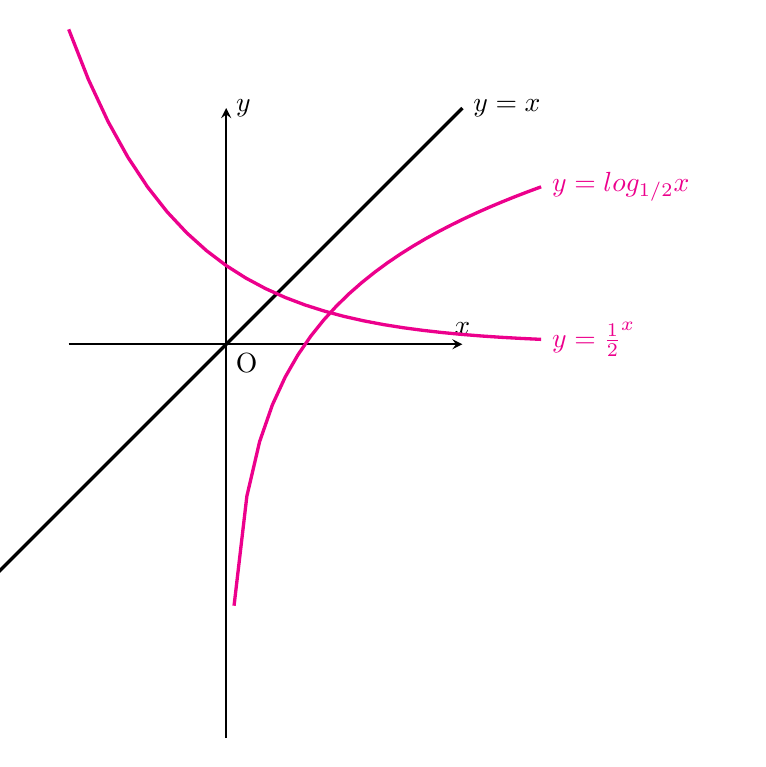
\begin{tikzpicture}
  \draw[->,>=stealth,semithick] (-2,0)--(3,0)node[above]{$x$}; %x軸
  \draw[->,>=stealth,semithick] (0,-5)--(0,3)node[right]{$y$}; %y軸
  \draw (0,0)node[below right]{O}; %原点
  \draw (-1,1)node[below]{};
  \draw[very thick,domain=-3:3] plot(\x,{(\x)})node[right]{$y=x$};
  \draw[magenta,very thick,domain=0.1:4] plot(\x,{log2(\x)})node[right]{$y=log_{1/2}{x}$};
  \draw[magenta,very thick,domain=-2:4] plot(\x,{0.5^(\x)})node[right]{$y=\frac{1}{2}^x$};
 \end{tikzpicture}

 \begin{tikzpicture}
  \draw[->,>=stealth,semithick] (-3,0)--(3,0)node[above]{$x$}; %x軸
  \draw[->,>=stealth,semithick] (0,-1)--(0,5)node[right]{$y$}; %y軸
  \draw (0,0)node[below right]{O};
  \draw (0,4)node[above right]{4};
  \coordinate [label=left:2] (A) at (0,2);
  \foreach \P in {A} \fill[black] (\P) circle (0.06);
  \draw(0,2) circle (2);
 \end{tikzpicture}

 \begin{tikzpicture}
 \tikz\draw(0,0)--(6,0)--(6,5)--cycle;
 \draw (0,0)node[above right]{x};
 \end{tikzpicture}
\end{document}
